\input{defs}

\newcommand{\draftpaper}{}
\newcommand{\revision}{}

\emergencystretch=\hsize
\lefthyphenmin=2
\righthyphenmin=2
\tolerance=9999

% detect interpreter: pdflatex or latex

\newif\ifpdf
\ifx\pdfoutput\undefined
  \pdffalse
\else
  \pdftrue
\fi

\newif\iflong
\ifx\longpaper\undefined
  \longfalse
\else
  \longtrue
\fi

\newif\ifdraft
\ifx\draftpaper\undefined
  \draftfalse
\else
  \drafttrue
\fi

\newif\ifverbose
\ifx\verbosepaper\undefined
  \verbosefalse
\else
  \verbosetrue
\fi

%
% REVCHANGE
%
\newif\ifrev
\ifx\revision\undefined
  \revfalse
\else
  \revtrue
\fi

% use document class IROS with any paper size:

%%\iflong
%%  \documentclass[a4]{epirob}
  \documentclass[]{article}
%%\else
%%  \documentclass[a4paper]{IROS}
%%\fi

	 \usepackage{fancyhdr}
	 \usepackage{fullpage}

\lhead[\fancyplain{}{}]       {\fancyplain{}{}}
\rhead[\fancyplain{}{\thepage}]       {\fancyplain{}{\thepage}}
\renewcommand{\headrulewidth}{0pt}
%
%	\addtolength{\oddsidemargin}{-.875in}
%	\addtolength{\evensidemargin}{-.875in}
%	\addtolength{\textwidth}{1.75in}

%	\addtolength{\topmargin}{-.875in}
%	\addtolength{\textheight}{1.75in}

\usepackage{pf-mod}

\usepackage{natbib}

\usepackage[nolists,tablesfirst]{endfloat}


\renewcommand{\cite}{\citep}


%%\documentclass[a4paper]{article}

%%\documentstyle{doublespace}



\ifpdf
  \usepackage{graphicx}
\else
  \usepackage[dvips]{graphicx}
\fi

\usepackage{psfig}

%%\setlength{\baselinestretch}{1.62}

%5\usepackage{setspace}
%%\setstretch{2.0}
\usepackage{doublespace}

\usepackage{pf-mod}

%\let\Caption\caption
%\renewcommand\caption[1]{%
%    \Caption[#1]{}%
%}

\begin{document} 



\onecolumn


% create the title header:
\ifrev
\title{Better Vision Through Manipulation}
\else
\title{Early Integration of Vision and Manipulation}
\fi

\author{
Giorgio Metta\\
LIRA-Lab, DIST\\
University of Genova\\
Genova, Italy\\
{\tt pasa@dist.unige.it}
\and 
Paul Fitzpatrick\\
Artifical Intelligence Lab\\
Massachusetts Institute of Technology\\
Cambridge, MA, USA\\
{\tt paulfitz@ai.mit.edu}
}

%%\iflong
%%  \author{Giorgio Metta$^{*,**}$
%%        \and
%%         Paul Fitzpatrick$^{**}$}
%%  \affiliation{\rm $^{*}$LIRA-Lab, DIST \\
 %%              University of Genova \\
 %%               Viale F. Causa, 13 \\
  %%              16145 Genova, Italy \\
  %%         \and
 %%             $^{**}$MIT AI Lab\\
 %%            200 Technology Square \\
 %%            Cambridge, MA 02139 US }
%%\else
%%\author{Paul M. Fitzpatrick$^{*}$ and Giorgio Metta$^{*,\dagger}$}
%%\affiliation{
%%$^{*}$MIT AI Lab -- Massachussetts Institute of Technology -- USA\\
%%$^{\dagger}$Lira Lab, DIST -- University of Genova -- Italy
%%}
%%\fi

%%\maketitle\thispagestyle{empty} % don't forget \thispagestyle{empty}, otherwise you'll get page numbering


\faketitle\thispagestyle{empty}

\vskip 3em%

Address correspondence to ONE OF US (phone ONE-OF-OUR-PHONES, fax
ONE-OF-OUR-FAXES).

\clearpage

\thispagestyle{empty}

{
\newcommand{\shorten}{use this option to shorten the abstract (200 words max)}


\iflong
\begin{abstract}
\else
\begin{Abstract}
\fi
 
Vision and manipulation are inextricably intertwined in the primate
brain.  Tantalizing results from neuroscience are illuminating the
mixed representations used by the brain in reaching, grasping, and
object recognition.  We wish to instantiate these results in robotic
form to probe their technical advantages and verify that the
associated models are at least consistent and without lacunae.

We believe it would be missing the point to investigate this on a
platform where dextrous manipulation and sophisticated machine vision
are already implemented (if such a platform existed).

In this paper, we show how we can take a simple precursor to manipulation,
namely poking and prodding, and already realize significant advantages in
visual processing, and make enough progress to develop a system that
is functionally analogous to models coming out of neuroscience.

We show how operational concepts can actually lead to well grounded
objects.


\ifverbose
For the purposes of manipulation, we would like to know what parts of
the environment are physically coherent ensembles -- that is, which
parts will move together, and which are more or less independent.  It
takes a great deal of experience before this judgement can be made
from purely visual information.  This paper develops active strategies
for acquiring that experience through experimental manipulation, using
tight correlations between arm motion and optic flow to detect both
the arm itself and the boundaries of objects with which it comes into
contact.  We argue that following causal chains of events out from
the robot's body into the environment allows for a very natural
developmental progression of visual competence, and relate this idea 
to results in neuroscience.
\fi

\ifverbose
For the purpose of understanding development we would like to present
causality as a possible principle to frame a number of neural science
results coherently. We will show how this can lead also to an
implementation in an artificial system following the epigenetic
approach. To this purpose we will show different levels of causal
linkages, or instances of the general principle, which allow tasks of
increasing complexity to be implemented.  Action and the physical
interaction of the robot with the environment play a fundamental role.
In an ecological perspective, the role of this physical interaction
for developing categorization and object undestanding is emphasized.
\fi

%%{\bf \em
%%\iflong
%%(long version)
%%\else
%%(short version)
%%\fi
%%}

\iflong
\end{abstract}
\else
\end{Abstract}
\fi


\begin{center}
{\bf keywords: } humanoid robotics, active segmentation, epigenesis
\end{center}

\begin{center}
{\bf running title: } Vision and Manipulation
\end{center}

}




\clearpage


\maketitle

\ifdraft
  \pagenumbering{arabic}
  \thispagestyle{plain}
  \pagestyle{plain}
\fi

\pagestyle{fancy}

% write the abstract with the Abstract-environment:

\iflong
\begin{abstract}
\else
\begin{Abstract}
\fi
 
Vision and manipulation are inextricably intertwined in the primate
brain.  Tantalizing results from neuroscience are illuminating the
mixed representations used by the brain in reaching, grasping, and
object recognition.  We wish to instantiate these results in robotic
form to probe their technical advantages and verify that the
associated models are at least consistent and without lacunae.

We believe it would be missing the point to investigate this on a
platform where dextrous manipulation and sophisticated machine vision
are already implemented (if such a platform existed).

In this paper, we show how we can take a simple precursor to manipulation,
namely poking and prodding, and already realize significant advantages in
visual processing, and make enough progress to develop a system that
is functionally analogous to models coming out of neuroscience.

We show how operational concepts can actually lead to well grounded
objects.


\ifverbose
For the purposes of manipulation, we would like to know what parts of
the environment are physically coherent ensembles -- that is, which
parts will move together, and which are more or less independent.  It
takes a great deal of experience before this judgement can be made
from purely visual information.  This paper develops active strategies
for acquiring that experience through experimental manipulation, using
tight correlations between arm motion and optic flow to detect both
the arm itself and the boundaries of objects with which it comes into
contact.  We argue that following causal chains of events out from
the robot's body into the environment allows for a very natural
developmental progression of visual competence, and relate this idea 
to results in neuroscience.
\fi

\ifverbose
For the purpose of understanding development we would like to present
causality as a possible principle to frame a number of neural science
results coherently. We will show how this can lead also to an
implementation in an artificial system following the epigenetic
approach. To this purpose we will show different levels of causal
linkages, or instances of the general principle, which allow tasks of
increasing complexity to be implemented.  Action and the physical
interaction of the robot with the environment play a fundamental role.
In an ecological perspective, the role of this physical interaction
for developing categorization and object undestanding is emphasized.
\fi

%%{\bf \em
%%\iflong
%%(long version)
%%\else
%%(short version)
%%\fi
%%}

\iflong
\end{abstract}
\else
\end{Abstract}
\fi


% ...and start writing!


\section{Outline}

The sad fate of most robot software

Modularity in robotics

YARP: Yet Another Robot Platform

Excising communication ``plumbing'' from code

Excising device dependencies from code

Conclusions


\section{Sad fate}

Many robot projects are ``black holes'', in terms of software.  A lot
of software gets sucked in, but very little comes out.  Once a piece
of software has been adapted to a particular robot, it takes a lot
of work to extricate it again and apply it to another.

Obviously the answer to this problem is modularity.  So there are 
now many architectures/frameworks/... for modular robot systems.
The prime concern for any such system should be that it is not
a ``black hole'' -- that once a piece of software has been adapted
to a particular framework, it takes a lot of work to extricate it
again and apply it to another.  That would be a bit self-defeating.

We study YARP from this perspective.  How sticky is resultant user
code to the robot and to the framework itself?


\section{Free and Open Source}

Useful, more malleable.

Has the pragmatic benefit that a user of the software can
modify and integrate it to their hearts content without the 
pain of dealing with opaque binaries.

Has the revolutionary benefit that the user is not trapped in the role
of being a ``consumer'' of software, but can also be a publisher of
the changes, additions, and integrative work they do in an effective
form.  This is achieved by explicitly granting far more rights to
users than they have under the law of most countries, contrasting with
agreeably with the formerly more common practice of attempting to
minimize user rights.  These rights are typically granted
conditionally; a user may only make use of these extended rights if
(for example) distributed code is always available in its most useful
original (source) form, with compatible freedoms attached to it.  This
condition seeks to balance freedoms of individuals versus benefit to
the group.  The freedom to distribute code in obscure (compiled) forms



Split between people who emphasize pragmatic concerns and those
who emphasize freedom.  Just cite the issue, no need to revisit
it here.


\section{CMake}

Open-source, deals well with various IDEs and command-line development.

Not as familiar as autoconf/automake/... etc.

Has the excellent property of being simpler than making Makefiles
or configuring a project, when external libraries are involved.

The big downside is that the language is unfamiliar and a bit ugly.
It is simple and well-documented, but quirky.  An alternative with
some similar properties, scons, uses python instead.  The ant system
uses with java also seems cleaner.  However, it gets the job
done, and has the huge advantage of not being dependent on an
external language being installed.

CMake is free and open-source, with a healthy community of 
developers.



\section{Call for publication}

As a research community, we both read and produce papers, building on
each others' work.

We also both acquire and produce software

Our software tends to die with our projects

Sad!  Software collaboration speeds things up

Research groups that all use a specific robot (Khepera, Pioneer, AIBO,
...) often form a natural software community

But each alone is a small subset of robotics

Groups developing new robots face obstacles

Differences in sensors, actuators, bodies...

Differences in processors, operating systems, libraries, frameworks,
languages, compilers...

Big barriers to software collaboration


\section{Modularity}

Constant hardware flux

Parts change rapidly

Interfaces change slowly

Lots of software grew and evolved alongside the changing hardware

Parts change rapidly

Interfaces change slowly

``Modularity'' is rewarded


\subsection{Broom}

The way parts interact can last longer than the parts themselves

E.g. an eternal broom

replace broom head

replace broom handle


\subsection{Theseus}

Long-lived software is like the Ship of Theseus

The mast gets replaced

The planks get replaced

Over time, everything may get replaced

In philosophy, this is a ``paradox of identity''

For us, it's just our job


\subsection{dark path}

The opposite of a modular system is a coupled one.

In a ``coupled'' system, changes in one part trigger changes in another.

Coupling leads to complexity

Complexity leads to confusion

Confusion leads to suffering

This is the path to the Dark Side

\subsection{modular robots}

Robot software is notoriously hardware-specific and task-specific

Both hardware and target tasks change quickly, even within the
lifetime of one project

Our humanoid robots are far more complex than one person can build and
maintain, both in terms of hardware and software

They need to be modular


\subsection{YARP}

YARP is an open-source software library  for humanoid robotics

History

An MIT / LIRA-Lab collaboration

Born on Kismet, grew on COG

With a major overhaul, now used by RobotCub consortium

Exists as an independent open source project

C++ source code


\subsection{Things we use}

CMake slide.

SWIG slide.


\subsection{What is YARP for}


Factor out details of data flow between programs from program source code

Data flow is very specific to robot platform, experimental setup,
network layout, communication protocol, etc.

Useful to keep ``algorithm'' and ``plumbing'' separate

Factor out details of devices used by programs from program source code

The devices can then be replaced over time by comparable alternatives;
code can be used in other systems


\section{Literature}

The literature of a research community both expresses its ideas, and
aids in their evolution

Published ideas are read, evaluated, and built upon

Useful advances get published

Publication of software can speed progress

Facilitates evaluating and comparing approaches

Brings new research topics into reach

Publish or perish!





\begin{figure}[tbh]
\centerline{
%%\includegraphics[width=\columnwidth]{cog-schematic.eps}
\includegraphics[width=6.0cm]{cog-schematic.eps}
%%\psfig{file=cog-schematic.eps,height=2.5in,clip=,silent=}
}
\caption{ 
%
  Degrees of freedom (DOFs) of the robot Cog.  The arms terminate
  either in a primitive ``flipper'' or a four-fingered hand.  
\ifverbose
The hand
  is an independent research project by Matthew Marjanovi\'{c}, and
  will not be employed or described here.  
\fi
  The head, torso, and arms
  together contain 22 degrees of freedom.
%
}
\label{fig:cog-schematic}
\end{figure}

\section{Our experimental platform}

\label{sect:robot}

\ifverbose
%
\begin{figure}[tbh]
\begin{center}
\includegraphics[width=5.0cm]{arm-motors.eps}
\caption{ 
\label{fig:arm-motors}
%
Kinematics of the arm, following \protect\cite{williamson99robot}.
There are a total of six joints, divided into a pair for each of
the shoulder, elbow, and wrist/flipper.
%
}
\end{center}
\end{figure}
%
\fi

This work is implemented on the robot Cog, an upper torso humanoid
\cite{brooks99cog}.  
%%The robot has previously been applied to tasks
%%such as visually-guided pointing \cite{Marjanovic-96-SAB}, and
%%rhythmic operations such as turning a crank or driving a slinky
%%\cite{williamson98neural}.  
Cog has two arms, each of which has six
degrees of freedom. %% -- two per shoulder, elbow, and wrist.
%% (see Figure~\ref{fig:arm-motors}).  
The joints are driven by series elastic
actuators \cite{williamson99robot}.
%% -- essentially a motor connected
%%to its load via a spring (think strong and torsional rather than
%%loosely coiled).  
The arm is not designed to enact trajectories with
high fidelity.  For that a very stiff arm is preferable.  Rather, it
is designed to perform well when interacting with a poorly
\ahhcharacterize{}d environment, where collisions are frequent and
informative events.
Cog runs an attentional system consisting of a set of pre-attentive
filters sensitive to motion, \ahhcolor{}, and binocular disparity. The
different filters generate information on the likelihood that
something interesting is happening in a certain region of the image. A
voting mechanism is used to ``decide'' what to attend and track
next. The pre-attentive filters are implemented on a space-variant
imaging system, which mimics the distribution
of photoreceptors in the human retina as in \cite{sandini-tagliasco-1980}.
 The attentional system uses vision and non-visual sensors
(e.g. inertial) to generate a range of oculomotor \ahhbehavior{}s. Examples
are saccades, smooth pursuit, vergence, and the vestibulo-ocular
reflex (VOR).








\input{section-where}

\begin{figure}[tb]
\begin{center}
\includegraphics[width=\columnwidth]{poking-sequence.eps}

%%\includegraphics[width=\textwidth]{poking-sequence.eps}
%%\includegraphics[width=14cm]{poking-sequence.eps}
\caption{ 
\label{fig:poking-sequence}
%
  The upper sequence shows an arm extending into a workspace, tapping
  an object, and retracting.  This is an exploratory mechanism for
  finding the boundaries of objects, and essentially requires the arm
  to collide with objects under normal operation, rather than as an
  occasional accident.  The lower sequence shows the shape
  identified from the tap using simple image differencing and flipper
  tracking.
%
}
\end{center}
\end{figure}



\section{Perceiving actions on objects}

Now that the robot knows something about its arm, it can start
to use it to explore its environment.
When the arm enters into contact with an object, one of several
outcomes are possible.  If the object is large, heavy, or otherwise
unyielding, motion of the arm may simply be resisted without any
visible effect.  Such objects are of little interest, except in their
role as obstacles, since the robot will not be able to manipulate
them.  But if the object is smaller, it is likely to move somewhat in
response to the nudge of the arm.  This movement will be temporally
correlated with the time of impact, and will be connected spatially to
the end-effector -- constraints that are not available in passive
scenarios~\cite{birchfield99depth}.  If the object is reasonably
rigid, and the movement has some component in parallel to the image
plane, the result is likely to be a flow field whose extent reflects
the physical boundaries of the object.  This visible response to
the robot's action can be used to refine its model of the object's
extent, which may be inaccurate.  For the example scene in
Figure~\ref{fig:setup-sequence} (a cube sitting on a table), the small
inner square on the cube's surface pattern might be selected as a
target.  The robot can certainly reach towards this target, but
grasping it would prove difficult without a correct estimate of the
object's physical extent.  In this section we show how the robot can
experimentally determine an object's extent using the same idea of
correlated motion used earlier to detect its own arm.

\subsubsection*{Making an impact}

Figure~\ref{fig:poking-sequence} shows how a ``poking'' movement can
be used to refine a target.  During this operation, the arm begins
by extending outwards from the resting position.  
\ifrevised
For this simple motivating example, the
\else
The 
\fi
end-effector (or
``flipper'') is local\ize{}d as the arm sweeps rapidly outwards using
the heuristic that it lies at the highest point of the region of optic
flow swept out by the arm in the image (the head orientation and
reaching trajectory are controlled so that this is true).  The arm is
driven outward into the \ahhneighbor{}hood of the target which we wish to
define, stopping if an unexpected obstruction is reached.  If no
obstruction is met, the flipper makes a gentle sweep of the area
around the target.  This minim\ize{}s the opportunity for the motion of
the arm itself to cause confusion; the motion of the flipper is
bounded around the endpoint whose location we know from tracking
during the extension phase, and can be subtracted easily.  Flow not
connected to the end-effector can be ignored as a distractor.


The sequence shown in Figure~\ref{fig:poking-sequence} is about the
simplest case possible for segmenting the motion of the object, since most of the arm is stationary
when contact occurs.  
In \ahhpractice{}, we would rather have less
constraints on the motion of the arm, so we can approach the object
from any convenient direction.  We found that it was possible 
to attain this flexibility without losing the simplicity of object
segmentation that poking brings, by exploiting the unique
visual opportunity afforded by the moment of impact,
as described in the next section.
%
\ifrevised
%
Another important question is, where does the target for poking come
from?  This is in fact very straightforward.  As described in
Section~\ref{sect:robot}, Cog has an attentional system that allows it
to locate and track salient visual stimuli.  This is based entirely on
low-level features such as color, motion, and binocular disparity that
are well defined on small patches of the image, as opposed to features
such as shape, size, and pose which only make sense on well-segmented
objects.  If Cog's attention system locates a patch of the image
that seems reachable (based on disparity and overall robot pose)
it will reach toward it and attempt to poke it so that
it can determine the physical extent of the object to which
that patch belongs.  A human can easily encourage this behavior
by bringing an object close to the robot, moving
it until the robot fixates it,
and then leaving it down on the table.  The robot will track the object
down to the table
(without the need or the ability to actually segment it),
 observe that it can be reached, and poke it.
%
\fi
%


\ifverbose
For simplicity, the head is kept steady throughout the poking
operation, so that simple image differencing can be used to detect
motion at a higher resolution than optic flow.  Because a poking
operation currently always starts from the same location, the arm
is local\ize{}d using a simple heuristic rather than the procedure described
in the previous section -- the first region of optic flow appearing
in the lower part of the robot's view when the reach begins
is assumed to be the arm.
\fi

\ifverbose
\begin{figure}[tbh]
\begin{center}
\includegraphics[width=\columnwidth]{cube-and-cylinder.eps}
\caption{ 
\label{fig:cube-and-cylinder}
%
  Poking can reveal a diffence in the shape of two objects without
  any prior knowledge of their appearance.
%
}
\end{center}
\end{figure}
\fi



\begin{figure}[tbh]
  \begin{center}
\includegraphics[width=\columnwidth]{fig-poke-zoom.eps}
%%    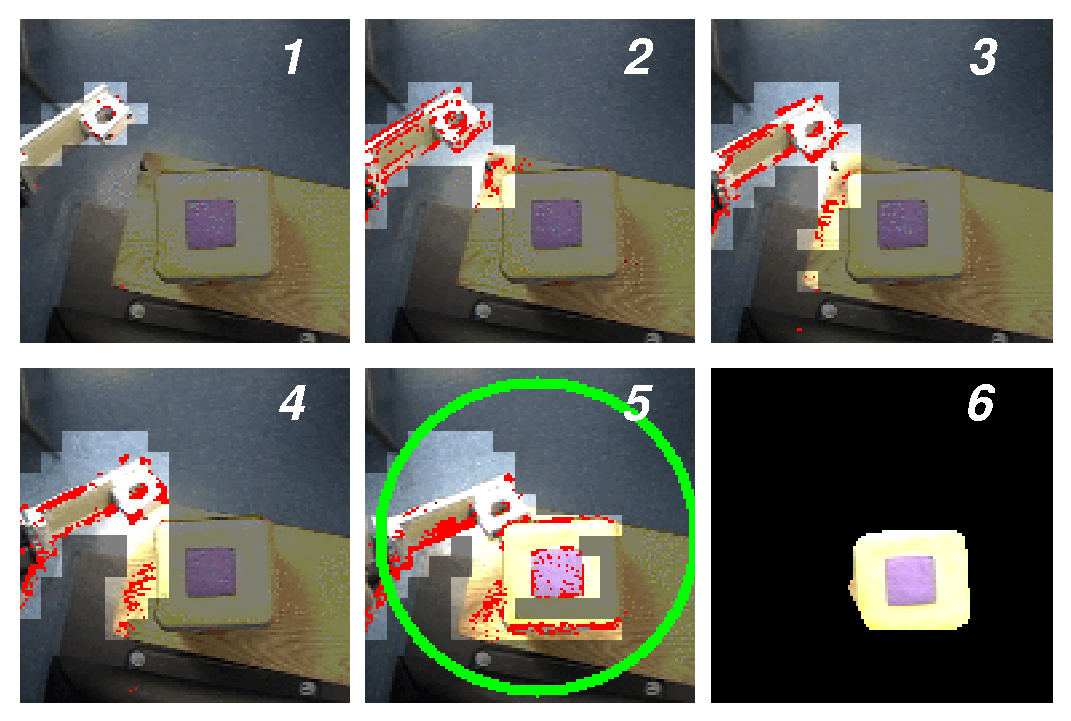
\includegraphics[width=8cm]{collision-detail}
  \end{center}
  \caption{
  \label{fig:poke-zoom}
    The moment of impact is detected visually by the
    sudden expansion of motion away from the arm.  Motion before and
    after contact is compared to gather information for segmentation.
}
\end{figure}


\subsubsection*{The moment of (ground) truth}

How can we detect when the arm collides with an object?  One natural
possibility would be to use proprioceptive or tactile information from
the arm itself.  Another possibility is to detect the collision
visually.  This is the method we use since, as
Section~\ref{sect:manipulator} will discuss, it allows collision
detection to be applied to human arm motion, a situation where the robot
does not have access to any privileged information about the motion.  When the robot 
is attempting to poke a target, it keeps the target fixated,
so that the image processing does not need to compensate for
egomotion.
Under these conditions, it is possible to detect motion using
image differencing.
This is a very simple technique for detecting motion by
simply subtracting successive frames coming from a camera and looking for
pixel-level differences.  A moving object that has some contrast with
the background it is moving over will generate such differences.  Of
course, pixel differences can also be generated by changes in
illumination, cast shadows, the refresh rate of computer monitors, movement of the camera
itself, etc.  A related technique called background mode\ling{} tries to
estimate the appearance of the fixed, stationary background of a 
scene, and then subtract the current view from the reference to 
detect new foreground.  Cog uses such a technique to detect motion
while it is fixating a target.

%% While these techniques are not ideally
%% suited to a moving platform like our robot, they are short periods 
%% during which they can be useful.  In particular, when the robot is
%% fixating a target, we can do this.

%%Two components -- detecting the moment of impact, and extracting as 
%%much data as possible from the frames around it.

%%There are particular periods when the robot is attentive and fixating.
%%When this is so, it can detect visually when a collision occurs
%%between a moving object and a previously stationary object in view.
%%The principal task, then, is keep the motion of the moving object distinct
%%from that of the impacted object.

%%Brief introduction to image differencing and background subtraction.
%%Stationary camera assumption to facilitate pixel modeling.  Don't want
%%to keep head stationary, but can fixate for significant periods.

Figure~\ref{fig:poke-zoom} shows the sequence of processing steps
taken as the arm approaches and comes into contact with a target.  As
the arm approaches, its motion is tracked very coarsely in real-time,
and areas it passes through are marked as ``clear'' of the object.  An impact event
is detected through a signature explosion of movement connected with
the arm, but spread across a much wider distance than the arm could
possibly have moved in the time available.  Once this impact is detected, we
start to process at high resolution (and drop briefly out of real-time
operation for a few seconds).  The raw motion signature generated by
the collision is computed.  The translational component of the arm
motion at the point of contact is also computed, so that motion present in
previous frames can be aligned with the collision frame, and motion 
associated with the arm can be isolated from motion
due to the target object.  Since the impact may occur just before a
frame is sampled (every 30 milliseconds) and so generate a relatively
weak motion signature, motion information from one frame after
collision is projected back and pooled with motion information in the
collision frame.  In the absence of strong texture there may be little apparent motion
 in the interior of the object, so we recruit a maximum-flow
algorithm due to \cite{boykov01experimental} to fill in such regions
efficiently.
%
Figure~\ref{fig:poking-segmentation} shows examples of segmentations
generated by very different poking operations -- one a gentle
tap from the side, the other a violent ``back-slap'' striking
the object away from the robot.

%%Within the context of the robot fixating a target, we try to detect
%%the moment of impact precisely, so we can apply the (relatively) slow
%%segmentation optimization to a narrow interval of the video input and
%%maintain close to real-time performance.  A moving manipulator
%%colliding with an object will accelerate it, if it is not too massive.
%%If the object is rigid, the motion of the manipulator will be transmitted 
%%through it.  This transmission can be detected as a spreading motion
%%that is not plausibly generated by the manipulator itself.

%%Some assumptions that may fail: object not too heavy; object at least
%%semi-rigid; manipulator not moving above a certain speed; manipulator
%%not casting shadows on the object itself.  When the robot is poking the
%%object itself, it can control some of this.  If the object iself is
%%troublesome, then we potentially diagnose this, or just ignore it.

%%We are relying on some facts about optic flow.  When an object is ...


%
\begin{figure}[tb]
\begin{center}
\includegraphics[width=10cm]{fig-poke-batting.eps}
%%\includegraphics[width=8cm]{segmentation-detail.eps}
%%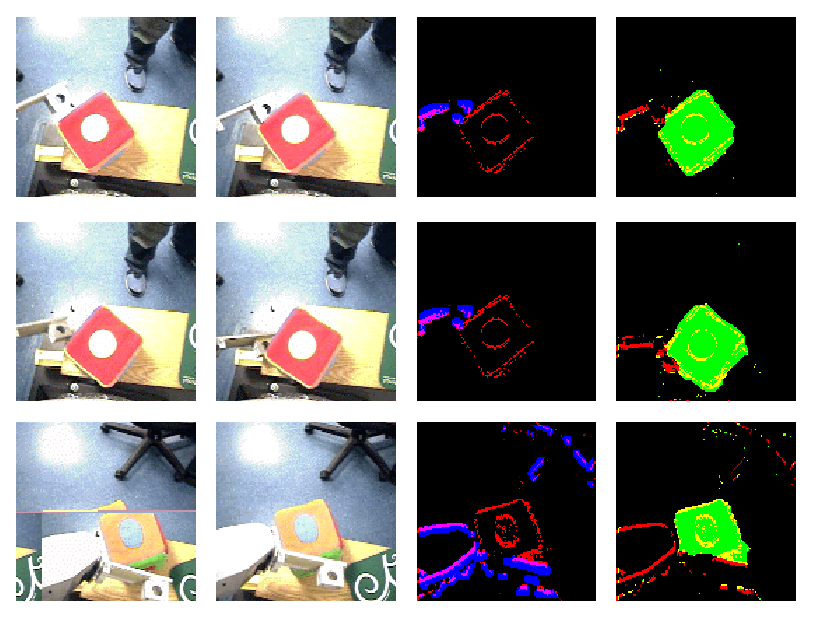
\includegraphics[width=\columnwidth]{poking_segmentation.eps}
\caption{ 
\label{fig:poking-segmentation}
%
Cog batting a cube around.  The top row shows the flipper poking
an object from the side, turning it slightly.  The second
row shows Cog batting an object away.  The images in the first column
are frames prior to a collision.  The second column shows the actual
impact.  The third column shows the motion signal at the point of
contact.  The bright regions in the images in the final column show
the segmentations produced for the object. 
%
}
\end{center}
\end{figure}
%




\subsubsection*{An operational definition of objecthood}

The poking operation gives clear results for a rigid object that is
free to move.  What happens for non-rigid objects and objects that are
attached to other objects?  Here the results of poking are likely to
be more complicated to interpret -- but in a sense this is a good
sign, since it is in just such cases that the idea of an object
becomes less well-defined.  Poking has the potential to offer an
operational theory of ``objecthood'' that is more tractable than a
vision-only approach might give, and which cleaves better to the true
nature of physical assemblages.  The idea of a physical object is
rarely completely coherent, since it depends on where you draw its
boundary and that may well be task-dependent.  Poking allows us to
determine the boundary around a mass that moves together when
disturbed, which is exactly what we need to know for manipulation.  As
an operational definition of object, this has the attractive property
of breaking down into ambiguity in the right circumstances~-- such as
for large interconnected messes, floppy formless ones, liquids, and so
on.  Poking also gives the robot the opportunity
to collect many views of a single object, and so we can hope to deal
with recogn\iz{}ing objects like the cube shown in
Figure~\ref{fig:sample-results}, which look different from every side.


\begin{figure}[tbh]
  \centerline{\includegraphics[width=9cm]{experiment-montage}}
  \caption{ 
  \label{fig:sample-results}
Results of a training session, where a toy cube was
  repeatedly offered to the robot for poking.  Each image of the cube
  corresponds to the segmentation found for it during a single poke.
  The most common failure mode is inclusion of the robot arm in the
  segmentation.  
}
\end{figure}




\section{Experimenting object affordances}

\ifverbose
The latest instantiation of the ``general principle'' we would like to
dwell upon is related to mirror neurons. It turns out that the causal
chain here is more compliceted. This requires a more complicated
structure to support it.
\fi

Poking moves us one step outwards on a causal chain away from the
robot and into the world, and gives a simple experimental procedure
for segmenting objects.  There are many possible elaborations of this
method, all of which lead to a vision system that is tuned to 
acquiring data about an object by seeing it manipulated by the robot.  

Segmentation alone is still unconvenient in many situation if not 
coupled with a mechanism to learn from experience. For example, it 
would be terribly unefficient to poke the object first and then try 
to grasp it. It would be much better if the robot could learn about
objects and [if it] had a way to identify a previously encountered object. 
A further difficulty, at least for a robot with a simple 
manipulator (e.g. as COG's flipper), is that ``affordances'' are scarce: 
most of the time the object simply move from one position
to another if we are willing to discount when it falls from the table.

However, for objects that roll there is a cue the robot can exploit
to understand their behavior. An object that rolls tends to do so even 
if it is not poked precisely. We selected a small set of objects to
experiment with: a cube, a toy car, an orange juice bottle, and a ball.
Affordances are not only a property of the mechanics of the object, but 
rather a combination of visual appearance, of the object's physical 
constituent, and of the ability of the actor. We selected a measure of
the principal axis of the object (easily obtained from the segmentation)
as visual component of the affordance. Table \ref{tab:affordances} shows the expected
behavior:

\begin{table*}[htbp]
\begin{center}
\begin{tabular}{|p{2cm}|p{3.5cm}|p{5cm}|}
\hline
{\it object} & {\it angle between principal axis and preferred direction of rolling} &  {\it behavior} \\ \hline\hline
{\bf cube} & n.a. & no principal axis, does not roll\\ \hline
{\bf car} & $0^\circ$ & rolls along the principal axis\\ \hline
{\bf bottle} &  $90^\circ$ & rolls at right angle\\ \hline
{\bf ball} &  n.a. & no principal axis, does roll\\ \hline
\end{tabular}
\caption{
\label{tab:affordances}
%
Behavior of a small set of objects when poked at random by the robot manipulator.
%
}
\end{center}
\end{table*}

A further elaboration is required to group the data belonging to the same
object as obtained from many poking acts into coherent clusters. As clustering 
mechanism we employed color histograms. After each poking action, a color histogram 
of the pixels of the segmented region is built and used as criterion 
to judge whether the object belongs to an existing group (i.e. if it
is mostly yellow, it is likely to be the toy car). This works well
for a limited set of objects but sophisticated methods are 
required for a more general case with many objects. 
The data structure that simulates the AIP-F5 affordance computation maintains all 
the instances of poking grouped by object, all the prototypes of the object segmented,
the direction of movement, and the action the robot applied in each particular case.

An alternative to the vision-based clustering procedure is to try to come 
to grips with the behavior of the objects after a single encounter, and use 
the behavior itself as clustering criterion. This is more difficult because 
of noise: e.g. there is still a non-zero probability that the object would 
not roll at all.

Figure \ref{fig:affordances} shows the results of the segmentation, clustering
and estimation of the affordance of the same set of four objects. The training set
consists of about 100 actions per object. The motor vocabulary of the robot
consists of four possible directions of poking. We labeled them for convenience
as: pull in, side tap, push away, and back slap, depending on the effect they
have on the object from the point of view of the robot. Actions were generated
at random during this training stage. During a poking action, the object is
tracked after the time of contact for 12 frames and the overall displacement is
estimated. 

\begin{figure}[tbh]
\begin{center}
\includegraphics[width=\columnwidth]{affordances.eps}
\caption{ 
\label{fig:affordances}
%
Probability of observing a roll along a particular direction for the set
of four objects used in our experiments. Abscissae represent the difference
between the principal axis of the object and the observed direction of 
movement. Ordinates the estimated probability.
%
}
\end{center}
\end{figure}

Yet this description of the affordances does not have any usable quantity to 
take action once an object is observed. For this purpose a description of 
the geometry of poking is required: i.e. the description of the properties of 
objects (figure \ref{fig:affordances}) has to be connected to a description
of the behavior of the object. 
This information can be derived from the same training set we collected for learning
about rolling. Figure \ref{fig:actions} shows the histograms of the direction 
of movement of the object for
each possible action. For example, the back slap moves the object mostly upward
(about $-100^\circ$) and away from the robot. A similar consideration applies
to the other poking gestures. Figure \ref{fig:actions} was obtained from the data of
about 500 poking events.

The last step is to connect all these elements together. If a known object is
presented to COG, the object is recognized, localized, and
its orientation estimated (principal axis). Recognition is based on the color histograms. The same
procedure used to form the clusters is employed here. Localization is simply implemented 
by histogram backprojection and a search across the image. The current orientation of the
object is then estimated by comparing the current image with all the prototypes 
contained in the cluster. The whole procedure gives a precision on the estimation
of the principal axis of about $10^\circ$ to $25^\circ$ depending on the object.  

To actually exploit the understanding of the affordance we need to connect vision to 
behavior. The robot looks for the preferred rolling direction of the object
(see figure \ref{fig:affordances}) and adds it to its current orientation. 
The action whose effects are closer (on average) to the last sum is selected.

% TEST OF PERFORMANCE MISSING?
We performed a simple qualitative test of the robot's behavior presenting randomly
two of the objects (the toy car and the bottle) - note that the ball and the cube 
do not have a well defined principal axis so there is no point in running the 
experiment. Out of 100 trials the robot made XY mistakes. Analysis 
of the errors reveals that they are mainly due to misinterpretation of the 
orientation of the object or to unprecise control.

\begin{figure}[tb]
\begin{center}
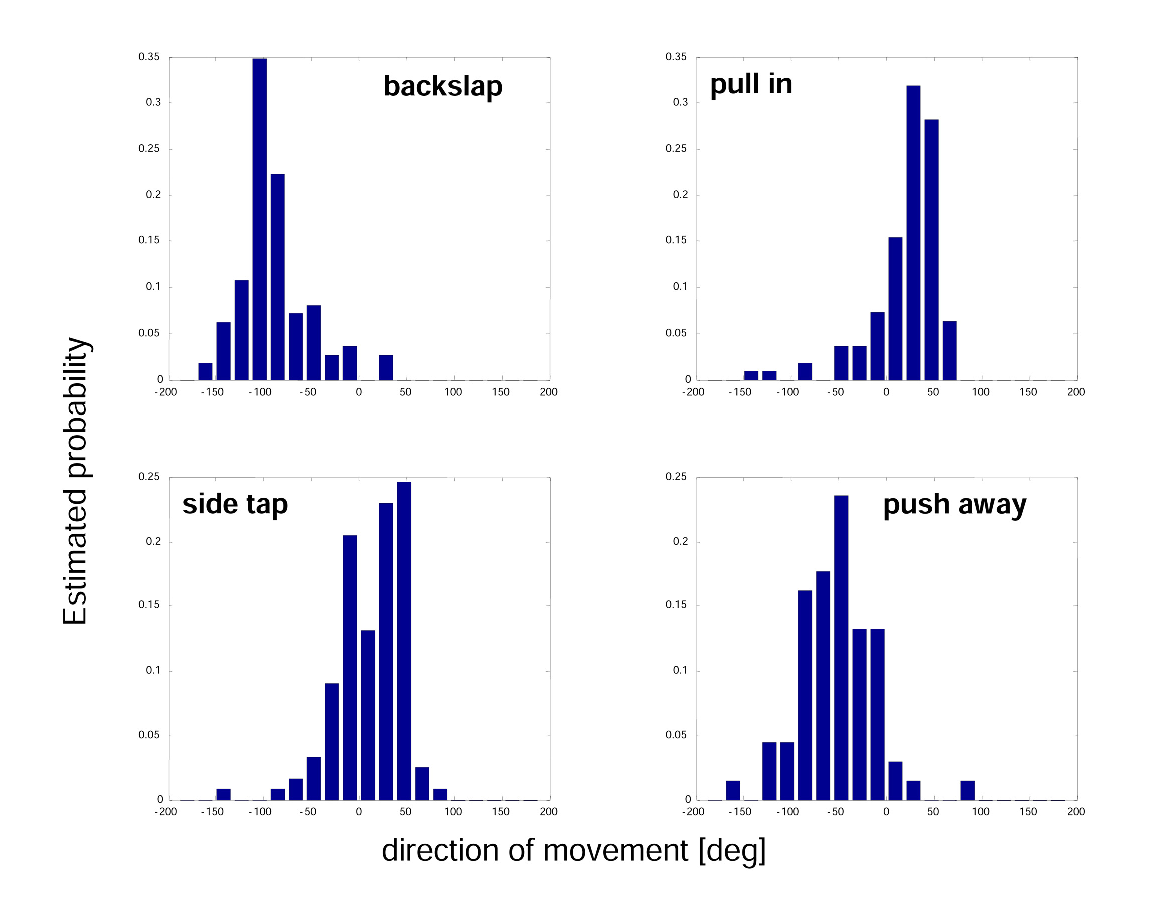
\includegraphics[width=12cm]{actions.eps}
\caption{ 
\label{fig:actions}
%
Histogram of the direction of movement of object for each possible poking action.
%
}
\end{center}
\end{figure}


\section{Developing mirror neurons}

\ifverbose
\begin{figure}[tb]
\begin{center}
\includegraphics[width=\columnwidth]{mirror-monkey.eps}
\caption{ 
\label{fig:mirror-monkey}
%
Mirror neurons and causality: from the observer's point
of view (A), understanding B's action means mapping it onto the
observer's own
motor repertoire. If the causal chain leading to the goal is already
in place (lower branch of the graph) then the acquisition of a
mirror neuron for this particular action/object is a matter of
building and linking the upper part of the chain to the lower one.
There are various opportunities to reinforce this link either at the object
level, at the goal level or both. 
%%Developmentally we can explain
%%mirror neurons only if we take into account another class of neurons
%%(called canonical) which in practice describes the lower branch of the
%%graph.
%
}
\end{center}
\end{figure}
\fi

An interesting question then is
whether the system could extract useful information from seeing an
object manipulated by someone else.  In the case of poking, the robot
needs to be able to estimate the moment of contact and to track the arm
sufficiently well to distinguish it from the object being poked.  We
are interested in how the robot might learn to do this.  One approach
is to chain outwards from an object the robot has poked.  If someone
else moves the object, we can reverse the logic used in poking --
where the motion of the manipulator identified the object -- and
identify a foreign manipulator through its effect on the object.






\ifverbose
Poking is an ideal testbed for future work on this, since it is much
simpler than full-blown object manipulation and would only require a
very simple model of the foreign manipulator to work.

There is considerable precedent in the literature for a strong
connection between viewing object manipulation performed by either
oneself or another \cite{wohlsclager02human}.  As we already mentioned
F5 contains a class of neurons called canonical neurons that have a
very specific response when an object is being either manipulated or
fixated.  Grossly simplifying, we might think of canonical neurons as
an association table of grasp/manipulation (action) types with object
(vision) types.  Another class of neurons called ``mirror neurons''
can then be thought of as a second-level association map which links
together the observation of a manipulative action performed by
somebody else with the neural representation of one's own action.

Figure~\ref{fig:mirror-monkey} shows this causal chain in action.
There are a series of interesting behaviors that can be realized based
on mirror neurons. Mimicry is an obvious application, since it
requires just this type of mapping between other and self in terms of
motor actions.  Another important application is the prediction of
future behavior from current actions, or even inverting the causal
relation to find the action that most likely will get to the desired
consequence.
\fi

\ifverbose

for example, by observing the part of an action the robot or the
bioagent can come out with suitable expectations of the consequences
of that action. On the other hand, the inverse behavior can also be
foreseen. The latter account to inverting the causal relation and
getting the action that most likely will get to the desired
consequence.

It might be argued that we need a two stages procedure to learn a
mirror representation, where we first learn ``something'' and only
subsequently we ``understand'' other people's behavior. The actual
developmental course might not be such artificially staged. A slight
advantage must be given though to the initial step of self-learning,
the undestanding comes later.


This set of associations can be learnt autonomously (by a robot for
example) simply by a trial and error procedure and possibly with a
reinforcing signal to tell when a given grasp/manipulatory gesture was
successful if applied to a particular object.

We should not probably think of this association as describing in
detail the object being manipulated visually. Perhaps only features
relevant to manipulation are stored (e.g. size, orientation in space).
This representation is a ``pragmatic'' one describing only those
properties of objects are needed to apply a particular set of actions
to them. Affordances are a good psychological analogue of F5
canonical neurons.
\fi


\ifverbose
How does this relate to causation?  The two situations in some sense
share the same goal, and more practically share the same object.  The
whole procedure assumes a basic discrimination of size and shape of
objects (not necessarily categorization in traditional sense), and the
exploitation of the visual information to the understanding of the
grasp type. In some cases though the goal might be unambiguous, e.g. a
needle is very unlikely grasped with a full palm grasp, as well as a
box is not grasped with a pinch grip. These are the most informative
allowing for the best discrimination of action type from the visual
perspective.
\fi

\ifverbose
The definition of imitation we gave here implicitly focus on imitating
the goal rather than the precise trajectory. This automatically takes
into account any difference in body structure between the actor and
the observer.

Of course, manipulation as in poking can lead to a better
understanding of the physical properties of objects not directly
amenable to visual exploration such as mass, roughness, softness, etc.
\fi

\begin{figure}[tbh]
\begin{center}
\includegraphics[width=\columnwidth]{mirror-cog.eps}
\caption{ 
\label{fig:mirror-cog}
%
The ultimate goal of this work is for our robot to follow chains of
causation outwards from its own simple body into the complex world.
%
}
\end{center}
\end{figure}





\section{Conclusions}

A bunch of stuff we should talk about...

A survey of robot development environments
\cite{kramer2007development} (p.s. rules YARP out, claim it has
no coherent program, think they were seeing YARP1).

% \cite{gerkey03player} % redundant to newer paper

% Not sure why this is here \cite{natale05developmental}

Nesnas \cite{nesnas2006claraty} - ``coping with hardware and software 
heterogeneity''.  It is useful for the list of problems it
works through (solutions are not that exciting).
%
Mentions danger of overgeneralizing interfaces, argues for 
``multi-level abstraction models, object-oriented methodologies
and design patterns''.  A bit vacuous.

Vaughan \cite{vaughan2006reusable} - this is a good player/stage
paper.

von Krogh \cite{vonkrogh2006promise} - looking at open source
software from a (management) research perspective.

Our previous comments on YARP1 \cite{metta2006yarp} which
describe its history and some usage information.

The case of embedded Linux \cite{henkel2006selective} --
interesting overlaps with robotics.

See Bill Gates article in Scientific American, January 2007

Missing infrastructure.
Need a lot of software.
Ideally (for researchers starting out) should be commoditized.


comparison with PC:

Difference: now we have the network.  Go the player route, rather than
the single IDE.  Transform from hardware to open protocols as first
step.  Then whole ecology of computation is available.

Robots aren't that special.  webcam/microphone/games...

The resources available to us are generally lower.  Smaller communities.
Less software expertise.  This could chage.







\subsection{YARP Network Scraps}

Not localization friendly, English bias at a quite low level.
Probably localization would not be practical at the network
protocol level.  Also approach to character encoding is
primitive and ad-hoc; no guarantee that encoded data
will survive in text-mode.



YARP is a free and open source project.  Since its source code is
released under a free and open license, useful parts of it can be used
by other systems, and its operation can be studied.

YARP has a large quantity of documentation (although we always need
more).  The communication protocol it uses is documented, and can be
interfaced with without using the YARP code-base.

Beyond just documenting the communication protocol, particular attention
has been devoted to make sure that that reading and writing data to a
YARP port can be done with very little effort.  YARP ports will 
accept and make connections of any of several different forms;
for a program build without the YARP code-base, it suffices
to implement just one of those connection types in order to
get basic connectivity.  If bandwidth requirements are not
excessive, the very simplest connection type can be implemented:
a very basic text-mode protocol.



% thanks to many people...

\input{section-acknowledgement}

% and the bibliography:

\newpage

%%\bibliography{abbreviations,biblio}
% **** PUT YOUR OWN BIBLIOGRAPHY FILES IN HERE ****
\bibliography{vision}



%\begin{figure}[tbh]
%  \begin{center}
%    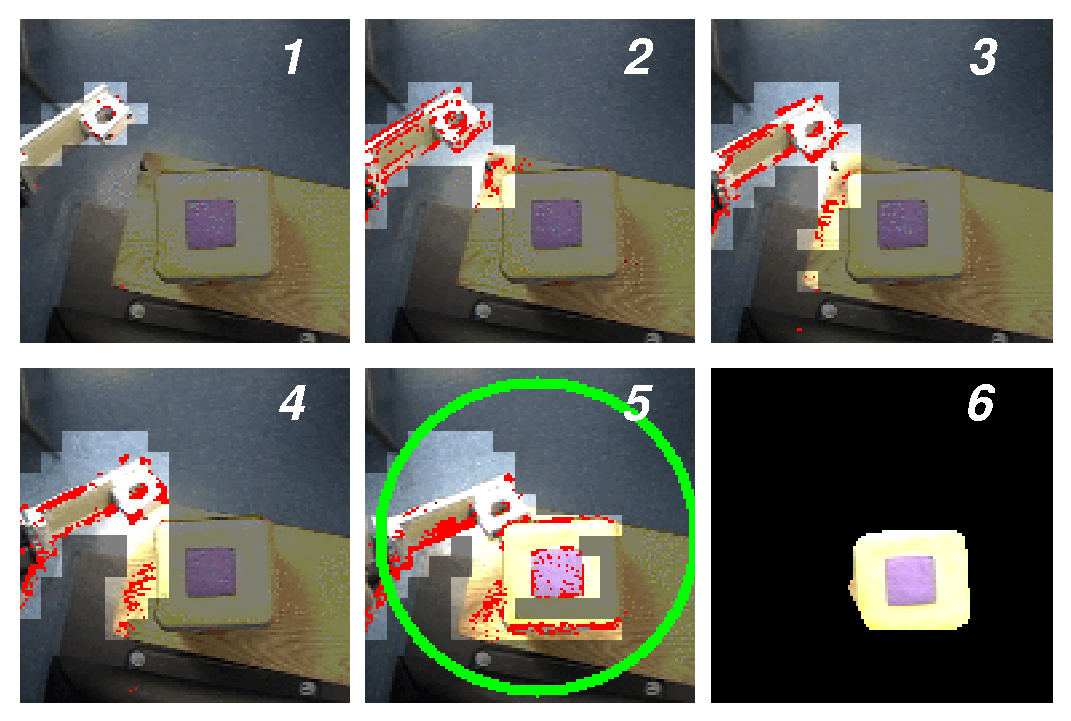
\includegraphics[width=2in]{collision-detail}
%    \hspace{1in}
%    \includegraphics[width=2in]{segmentation-detail}
%  \end{center}
%  \caption{Part of the process}
%\end{figure}

%\begin{figure}[tbh]
%  \centerline{\includegraphics[width=2.5in]{tracing_causes}}
%  \caption{foo} 
%  %%\label{fig:foo}
%\end{figure}

\begin{figure}[tbh]
  \centerline{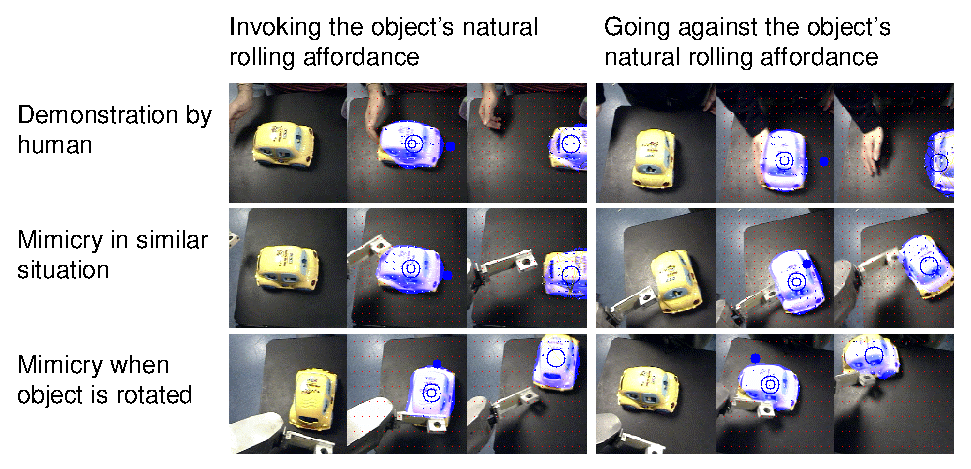
\includegraphics[width=\textwidth]{fig-mimicry-awkward}}
  \caption{foo} 
\end{figure}



\newpage

\listoftables

\newpage

\listoffigures




%% 
\section{Closing the loop}

%% rolling experiment

Poking is sufficient to explore some very simple affordances of
objects, such as rolling, toppling, breaking etc.  We explore the
rolling affordance with the four objects shown in
Figure~\ref{fig:rolling-motivate}.  Each of the objects rolls in a
different way, which the robot can learn about and exploit.

\begin{figure}[tbh]
  \centerline{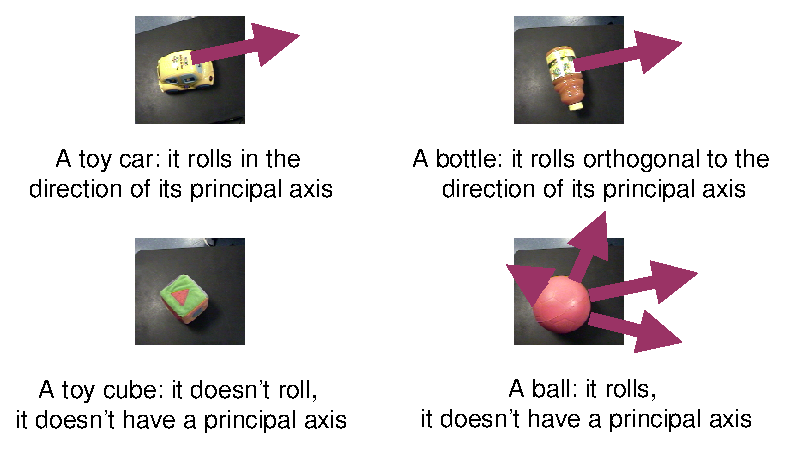
\includegraphics[width=12cm]{rolling-motivate}}
  \caption{
%
    Different objects roll in different ways.  A toy car rolls
    forward, a bottle rolls on its side, a sphere rolls in any
    direction, and a cube doesn't really roll at all.
%
} 
  \label{fig:rolling-motivate}
\end{figure}

\begin{figure}[tbh]
  \centerline{\includegraphics[width=12cm]{rolling-graphs}}
  \caption{
%
  The robot relates the direction an object moves in with the
  direction of its principal axis.  For a car, there is a clear
  tendency to roll in the direction of the principal axis.
  A bottle has a clear tendency to roll towards its side.
  Cars and spheres have no clear principal axis so, whether they
  roll or not, there is nothing to say.
%
} 
  \label{fig:rolling-graphs}
\end{figure}

The final behavior of the robot after training is: human presents an
object, makes it roll.  Presents the same object, perhaps in another
orientation, and the robot pushes it in the right direction to make it
roll.  If the human hits the object in a non-canonical direction,
so will the robot.  This serves to demonstrate the full loop of 
perception and action.






\end{document}

% and never mind LaTeX's hysterical warnings about missing fonts... everything's fine!
